\documentclass[12pt]{beamer}
\usetheme{Boadilla}
\usepackage{booktabs}
\usepackage{multirow}
\usepackage{enumitem}
\usepackage{tikz}

\newcommand{\E}{\mathbb{E}}
\usefonttheme{professionalfonts}
\usepackage{pgfplots}
\pgfplotsset{compat=1.18}
\renewcommand{\arraystretch}{1.25}
\usetikzlibrary{trees}
\title[ECON2843]{Lecture 23}
\subtitle{Part 5 Linear Regression}
\date{}
\usepackage{amsmath,amssymb,mathtools,wasysym}
\begin{document}
	\begin{frame}
		\titlepage
		
	\end{frame}
	\begin{frame}
		\vspace{1cm}
		\centering
		{\color{blue}\large Simple Linear Regression}
	\end{frame}
	
	


	\begin{frame}
		\frametitle{1. Checking the Model Assumptions}
		
		\begin{itemize}
			\item[\textcolor{blue}{(c)}] Certain plots can be used for checking the independence of the residuals, but if the sample is collected properly (i.e., randomly) this hopefully shouldn't be a major problem.
			\begin{itemize}[label={\color{blue}$\blacktriangleright$}]
				\item Can plot the residuals against the order in which the observations were collected to see if there is any time correlation between the residuals.
			\end{itemize}
		\end{itemize}
		
	\end{frame}
	\begin{frame}
		\frametitle{2. Testing Overall Significance of Model}
		
		\begin{itemize}[label={\color{blue}$\blacktriangleright$}]
			\item Once we are happy that the model assumptions are satisfied, the next thing we should do is test the \textit{overall significance} of the model.
			
			\item Testing the overall significance of the model is equivalent to testing whether or not a model exists.
			
			\item That is, does a linear relationship between $X$ and $Y$ even exist.
			
			\item How might we be able to test this?
		\end{itemize}
		
	\end{frame}
	\begin{frame}
		\frametitle{2. Testing Overall Significance of Model}
		
		\begin{itemize}[label={\color{blue}$\blacktriangleright$}]
			\item If $\beta_1 = 0$, what happens to the simple linear regression model?
			
			\item The model
			\[Y = \beta_0 + \beta_1X + \epsilon\]
			becomes
			\[Y = \beta_0 + \epsilon\]
			
			\item That is, $X$ disappears from the model, indicating that no linear relationship exists between $X$ and $Y$.
			
		\end{itemize}
		
	\end{frame}
	\begin{frame}
		\frametitle{Hypotheses}
		
		\begin{itemize}[label={\color{blue}$\blacktriangleright$}]
			\item The hypotheses for testing the overall significance of the simple linear regression model are:
			
			\[
			\begin{aligned}
				H_0 : \beta_1 &= 0 \\
				H_1 : \beta_1 &\neq 0
			\end{aligned}
			\]
			
			\item Note that we are testing the two-tailed alternative, since either $\beta_1 > 0$ or $\beta_1 < 0$ would indicate that a model exists.
			
		\end{itemize}
		
	\end{frame}
	\begin{frame}
		\frametitle{Test Statistic}
		
		\begin{itemize}[label={\color{blue}$\blacktriangleright$}]
			\item The test statistic that we use to test the above hypotheses is the $T$-statistic:
			
			\[
			T = \frac{\hat{\beta}_1 - 0}{s_{\hat{\beta}_1}} = \frac{\hat{\beta}_1}{s_{\hat{\beta}_1}}
			\]
			
			where $s_{\hat{\beta}_1} = \sqrt{\frac{1}{n-2}\sum_{i=1}^n e_i^2 \over (n-1)s_X^2}$ is an estimate of the standard error of $\hat{\beta}_1$ (i.e., the standard deviation of the sampling distribution of $\hat{\beta}_1$).
			
		\end{itemize}
		
	\end{frame}
	\begin{frame}
		\frametitle{Decision Rule}
		
		\begin{itemize}[label={\color{blue}$\blacktriangleright$}]
			\item For our decision rule, we need to compare this $T$-statistic to a $t$-distribution with $n-2$ degrees of freedom.
			
			\item Since it is a two-tailed test, we reject $H_0$ at a significance level of $\alpha$ if $T > t_{\frac{\alpha}{2},n-2}$ or $T < -t_{\frac{\alpha}{2},n-2}$.
			
		\end{itemize}
		
	\end{frame}
	\begin{frame}
		\frametitle{Example}
		
		\begin{itemize}[label={\color{blue}$\blacktriangleright$}]
			\item Let's go back to our example to test the overall significance of the model which had attitude as the dependent variable $Y$ and duration of residence as the independent variable $X$.
			
			\item Remember the hypotheses are:
			\[
			\begin{aligned}
				H_0 : \beta_1 &= 0 \\
				H_1 : \beta_1 &\neq 0
			\end{aligned}
			\]
			
			\item We can calculate the test statistic by hand or we can also use the computer output.
			
		\end{itemize}
		
	\end{frame}

	\begin{frame}[fragile]
		\frametitle{Example}

			\begin{verbatim}
				Call:
				lm(formula = attitude ~ duration, data = city.dat)
				
				Residuals:
				Min      1Q  Median      3Q     Max 
				-1.9262 -0.7640 -0.4579  0.6165  2.7494 
				
				Coefficients:
				Estimate Std. Error t value Pr(>|t|)
				(Intercept)  1.2237    1.0531    1.162 0.275114
				duration     0.5585    0.0952    5.867 0.000239


				Residual standard error: 1.493 on 9 degrees of freedom
				Multiple R-squared: 0.7927,  Adjusted R-squared: 0.7697
				F-statistic: 34.42 on 1 and 9 DF,  p-value: 0.0002387
		
		\end{verbatim}
	\end{frame}
	\begin{frame}
		\frametitle{Example}
		
		\begin{itemize}[label={\color{blue}$\blacktriangleright$}]
			\item The test statistic is calculated as:
			\[
			T = \frac{\hat{\beta}_1}{s_{\hat{\beta}_1}} = \frac{0.5585}{0.0952} = 5.867
			\]
			
			\item There were $n = 11$ observations in our sample, so we compare this to a $t$-distribution with $n - 2 = 9$ degrees of freedom.
			
			\item At a significance level of $\alpha = 0.05$, the rejection region is therefore $T > 2.262$ or $T < -2.262$.
			
		\end{itemize}
		
	\end{frame}
	\begin{frame}
		\frametitle{Example}
		
		\begin{itemize}[label={\color{blue}$\blacktriangleright$}]
			\item Since $5.867 > 2.262$, we reject $H_0$ and conclude that there is a significant linear relationship between $X$ and $Y$.
			
			\item Alternatively, the computer output also gives us the $p$-value for the \textit{two-tailed} alternative hypothesis.
			
			\item So we can reach the same conclusion by comparing the $p$-value of 0.000239 to $\alpha = 0.05$.
			
		\end{itemize}
		
	\end{frame}
	\begin{frame}
		\frametitle{Testing the Correlation Coefficient}
		
		\begin{itemize}[label={\color{blue}$\blacktriangleright$}]
			\item Recall that the correlation coefficient $\rho$ measured the strength of a linear relationship between two variables.
			
			\item We can also test the overall significance of the simple linear regression model by testing the following hypotheses:
			
			\[
			\begin{aligned}
				H_0 : \rho &= 0 \\
				H_1 : \rho &\neq 0
			\end{aligned}
			\]
			
		\end{itemize}
		
	\end{frame}
	\begin{frame}
		\frametitle{Testing the Correlation Coefficient}
		
		\begin{itemize}[label={\color{blue}$\blacktriangleright$}]
			\item The test statistic we use is based on the sample correlation coefficient $r$:
			
			\[
			T = \frac{r \times \sqrt{n-2}}{\sqrt{1-r^2}}
			\]
			
			\item For the decision rule, we again compare this $T$-statistic to a $t$-distribution with $n-2$ degrees of freedom and reject $H_0$ at a significance level of $\alpha$ if $T > t_{\frac{\alpha}{2},n-2}$ or $T < -t_{\frac{\alpha}{2},n-2}$.
			
		\end{itemize}
		
	\end{frame}
	\begin{frame}
		\frametitle{Testing the Correlation Coefficient}
		
		\begin{itemize}[label={\color{blue}$\blacktriangleright$}]
			\item Note that when testing $\beta_1 = 0$ in the simple linear regression model and when testing $\rho = 0$, both test statistics are compared to the same sampling distribution.
			
			\item These two tests are indeed equivalent, in the sense that some algebra can show:
			
			\[
			\frac{\hat{\beta}_1}{s_{\hat{\beta}_1}} = \frac{r \times \sqrt{n-2}}{\sqrt{1-r^2}}
			\]
			
		\end{itemize}
		
	\end{frame}
	\begin{frame}
		\frametitle{Testing the Correlation Coefficient}
		
		\begin{itemize}[label={\color{blue}$\blacktriangleright$}]
			\item For our city example data, the sample correlation coefficient between $X$ and $Y$ is $r_{XY} = 0.8903507$, so we get:
			
			\[
			\begin{aligned}
				T &= \frac{r \times \sqrt{n-2}}{\sqrt{1-r^2}} \\[2ex]
				&= \frac{0.8903507 \times \sqrt{11-2}}{\sqrt{1-0.8903507^2}} \\[2ex]
				&= 5.867
			\end{aligned}
			\]
		\end{itemize}
	\end{frame}
	\begin{frame}
		\frametitle{General Test for $\beta_1$}
		
		\begin{itemize}[label={\color{blue}$\blacktriangleright$}]
			\item Aside from testing the overall significance of the simple linear regression model, we can also test more general hypotheses regarding $\beta_1$:
			
			\[
			\begin{aligned}
				H_0 &: \beta_1 = c \\[2ex]
				H_1 &: \beta_1(\neq,<,>)c
			\end{aligned}
			\]
		\end{itemize}
	\end{frame}
	\begin{frame}
		\frametitle{General Test for $\beta_1$}
		
		\begin{itemize}[label={\color{blue}$\blacktriangleright$}]
			\item The test statistic takes on the usual form:
			
			\[
			T = \frac{\hat{\beta_1} - c}{s_{\hat{\beta_1}}}
			\]
			
			\item For the decision rule, we compare the test statistic to a $t$-distribution with $n-2$ degrees of freedom.
		\end{itemize}
	\end{frame}
	\begin{frame}
		\frametitle{General Test for $\beta_0$}
		
		\begin{itemize}[label={\color{blue}$\blacktriangleright$}]
			\item Although most interest in a simple linear regression usually concerns $\beta_1$, we can also test hypotheses regarding the intercept parameter $\beta_0$:
			
			\[
			\begin{aligned}
				H_0 &: \beta_0 = c \\[2ex]
				H_1 &: \beta_0(\neq,<,>)c
			\end{aligned}
			\]
		\end{itemize}
	\end{frame}
	\begin{frame}
		\frametitle{General Test for $\beta_0$}
		
		\begin{itemize}[label={\color{blue}$\blacktriangleright$}]
			\item The test statistic is:
			
			\[
			T = \frac{\hat{\beta_0} - c}{s_{\hat{\beta_0}}}
			\]
			
			where $s_{\hat{\beta_0}} = s_{\hat{\beta_1}} \times \sqrt{\frac{\sum_{i=1}^n X_i^2}{n}}$ is an estimate of the standard error of $\hat{\beta_0}$.
			
			\item For the decision rule, we again compare the test statistic to a $t$-distribution with $n-2$ degrees of freedom.
		\end{itemize}
	\end{frame}
	\begin{frame}
		\frametitle{3. Estimating $\sigma_\epsilon^2$}
		
		\begin{itemize}[label={\color{blue}$\blacktriangleright$}]
			\item Now that we have established that the overall model is significant, how good is our model?
			
			\item Recall that the error variable $\epsilon_i$ represents the difference between the $Y_i$ value of each observation and the straight line component of the regression model.
			
			\item Further, the model assumptions stated that $\epsilon_i \stackrel{iid}{\sim} N(0, \sigma_\epsilon^2)$.
		\end{itemize}
	\end{frame}
		\begin{frame}
		\frametitle{3. Estimating $\sigma_\epsilon^2$}
	\centering
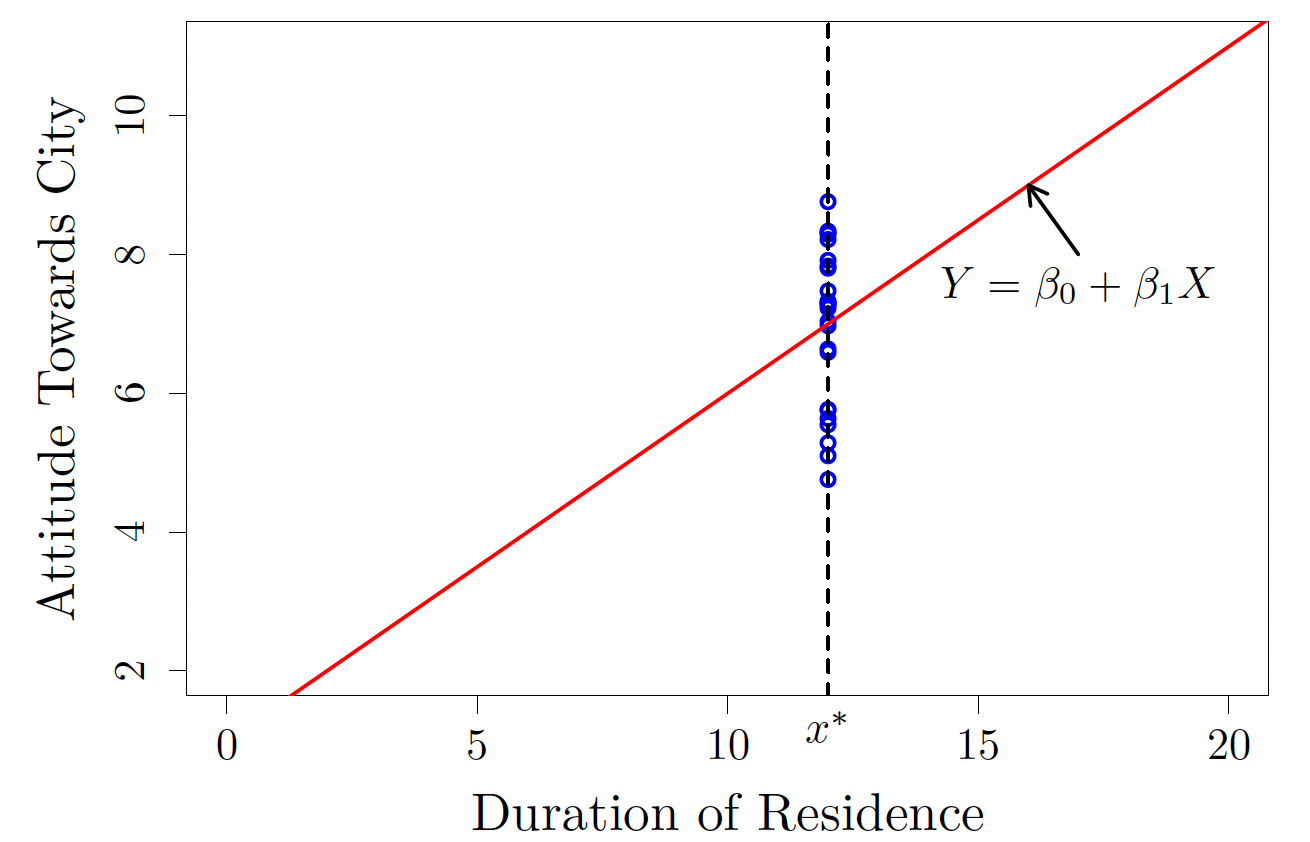
\includegraphics[width=12cm]{sigma.png}
\end{frame}
\begin{frame}
	\frametitle{3. Estimating $\sigma_\epsilon^2$}
	
	\begin{itemize}[label={\color{blue}$\blacktriangleright$}]
		\item If $\sigma_\epsilon^2$ is small, the errors $\epsilon_i$ are close to the mean 0, indicating that the regression model fits the data well.
		
		\item If $\sigma_\epsilon^2$ is large, some of the errors $\epsilon_i$ will be large, indicating that the regression model does not fit the data well.
		
		\item But $\sigma_\epsilon^2$ is an unknown population parameter, which therefore has to be estimated.
	\end{itemize}
\end{frame}
\begin{frame}
	\frametitle{3. Estimating $\sigma_\epsilon^2$}
	
	\centering
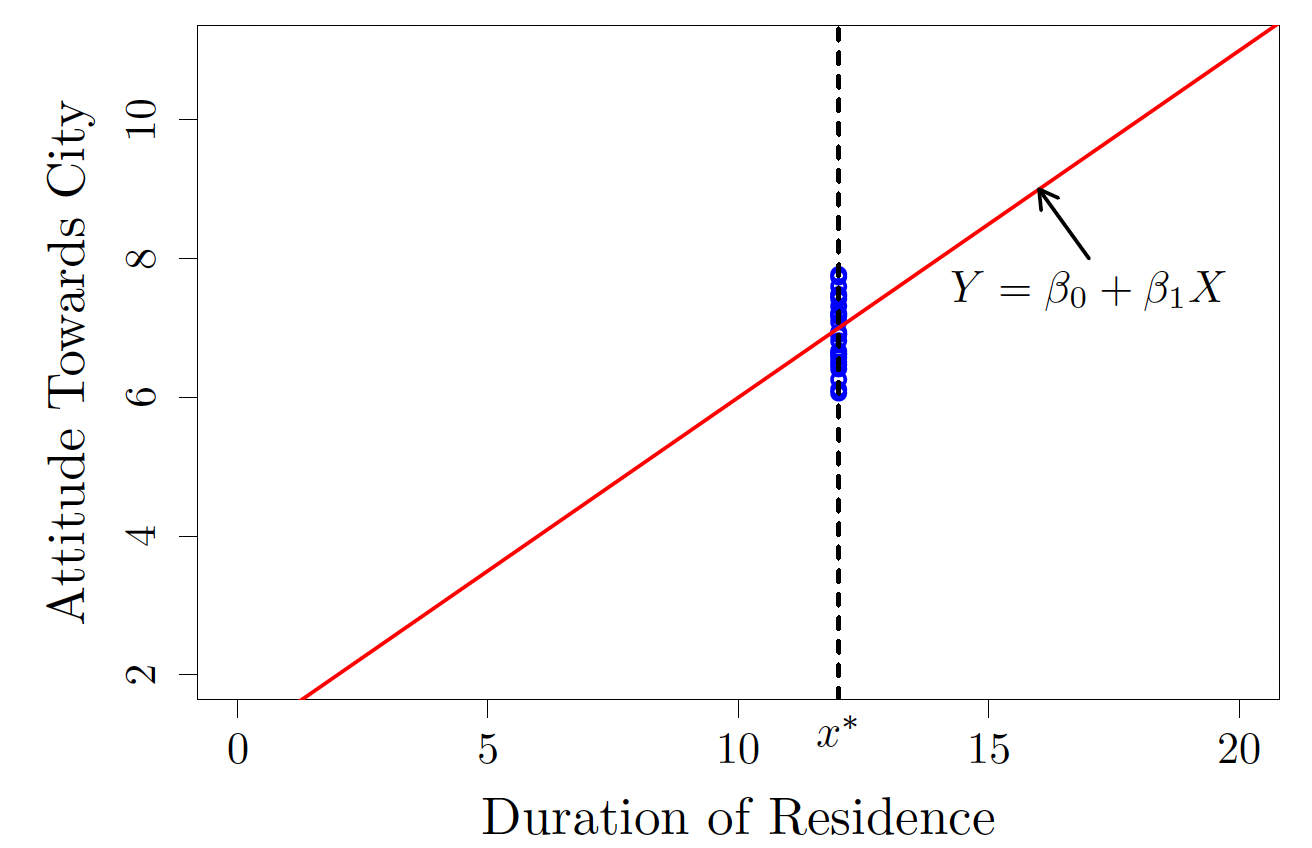
\includegraphics[width=12cm]{sigma2.png}
\end{frame}
\begin{frame}
	\frametitle{3. Estimating $\sigma_\epsilon^2$}
	
	\centering
	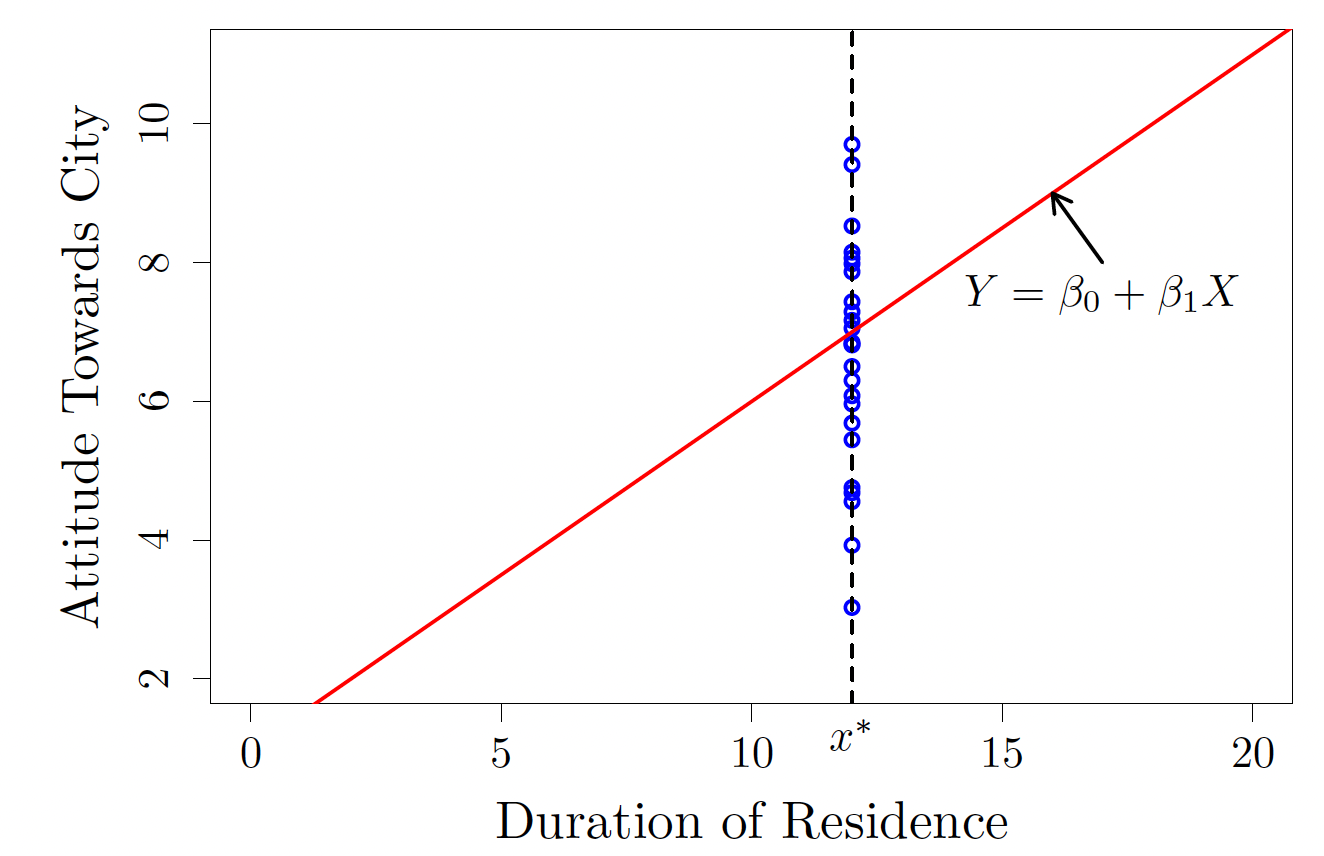
\includegraphics[width=12cm]{sigma3.png}
\end{frame}
\begin{frame}
	\frametitle{3. Estimating $\sigma_\epsilon^2$}
	
	\begin{itemize}[label={\color{blue}$\blacktriangleright$}]
		\item Again, since we don't know the true errors $\epsilon_i$, we use the residuals $e_i$ to obtain an \emph{unbiased} estimator of $\sigma_\epsilon^2$:
		
		\[
		s_\epsilon^2 = \frac{\sum_{i=1}^n e_i^2}{n-2} = \frac{\sum_{i=1}^n \left(Y_i - \hat{Y_i}\right)^2}{n-2}
		\]
		
		\item Note that $s_\epsilon$, the square root of $s_\epsilon^2$, is called the \textbf{standard error of estimate}.
	\end{itemize}
\end{frame}
\begin{frame}
	\frametitle{3. Estimating $\sigma_\epsilon^2$}
	
	\begin{itemize}[label={\color{blue}$\blacktriangleright$}]
		\item Just based on the value of $s_\epsilon^2$, it can be difficult to determine whether it's small enough to indicate a good model.
		
		\item However, it is useful for comparing two different models - the model with the smaller standard error of estimate is generally considered better.
	\end{itemize}
\end{frame}
\begin{frame}
	\frametitle{4. Calculating $R^2$}
	
	\begin{itemize}[label={\color{blue}$\blacktriangleright$}]
		\item If the overall model is significant, there exists a linear relationship between $X$ and $Y$.
		
		\item Would be nice to be able to measure the \emph{strength} of the linear relationship.
		
		\item This is measured by $R^2$, the \textbf{coefficient of determination}, and is defined by:
		
		\[
		R^2 = \frac{s_{XY}^2}{s_X^2 s_Y^2}
		\]
	\end{itemize}
\end{frame}
\begin{frame}
	\frametitle{4. Calculating $R^2$}
	
	\begin{itemize}[label={\color{blue}$\blacktriangleright$}]
		\item Note that $R^2$ is just the square of the sample correlation coefficient.
		
		\item There is also another way to express $R^2$, which is based on how much variation is explained by the regression model.
		
		\item Just like ANOVA, we can define some sums of squares\ldots
	\end{itemize}
\end{frame}
\begin{frame}
	\frametitle{Sums of Squares}
	
	\begin{itemize}[label={\color{blue}$\blacktriangleright$}]
		\item Total sum of squares:
		\[
		SS(Total) = \sum_{i=1}^n (Y_i - \bar{Y})^2
		\]
		
		\item Sum of squares for regression:
		\[
		SSR = \sum_{i=1}^n (\hat{Y_i} - \bar{Y})^2
		\]
		
		\item Sum of squares for error:
		\[
		SSE = \sum_{i=1}^n (Y_i - \hat{Y_i})^2
		\]
	\end{itemize}
\end{frame}
\begin{frame}
	\frametitle{4. Calculating $R^2$}
	
	\begin{itemize}[label={\color{blue}$\blacktriangleright$}]
		\item It is also true that:
		
		\[
		SS(Total) = SSR + SSE
		\]
		
		\item Some algebra will show that the coefficient of determination can also be written as:
		
		\[
		R^2 = \frac{SSR}{SS(Total)}
		\]
	\end{itemize}
\end{frame}
\begin{frame}
	\frametitle{4. Calculating $R^2$}
	
	\begin{itemize}[label={\color{blue}$\blacktriangleright$}]
		\item Therefore, $R^2$ also measures the proportion of total variation in $Y$ that is explained by the simple linear regression model.
		
		\item Similar to $s_\epsilon^2$, $R^2$ is useful for comparing different models.
	\end{itemize}
\end{frame}
\begin{frame}
	\frametitle{Using the Model}
	
	\begin{itemize}[label={\color{blue}$\blacktriangleright$}]
		\item Once we have assessed the simple linear regression model and concluded that it was appropriate for our data, we can proceed to use our estimated model.
		
		\item Suppose we have a new observation from the population with an $X$ value equal to $X = x_g$.
		
		\item Given this value $x_g$, we can \emph{predict} the value of $Y$ using our estimated model:
		
		\[
		\hat{y}_g = \hat{\beta_0} + \hat{\beta_1}x_g
		\]
	\end{itemize}
\end{frame}
\begin{frame}
	\frametitle{Point Estimate}
	
	\begin{itemize}[label={\color{blue}$\blacktriangleright$}]
		\item So $\hat{y}_g$ gives us a \emph{point estimate} for the value of $Y$ when $X = x_g$.
		
		\item However, it does not tell us anything about how close this predicted value is to the true value of $Y$.
		
		\item How can we address this problem?
		
		\item We can use an interval estimator!
		
		\item Before we derive some interval estimators, for a given value of $X = x_g$, there are actually two different quantities that we might be interested in estimating\ldots
	\end{itemize}
\end{frame}
\begin{frame}
	\frametitle{Point Estimate}
	
	\begin{enumerate}[label=\textcolor{blue}{\arabic*.}]
		\item The particular value of $Y$ for that particular observation with $X = x_g$, that is,
		\[
		y_g = \beta_0 + \beta_1x_g + \epsilon_g
		\]
		
		\item The \emph{expected value} of $Y$ for \emph{all} observations with $X = x_g$, that is,
		\[
		E(Y|X = x_g) = \beta_0 + \beta_1x_g
		\]
	\end{enumerate}
	
	\begin{itemize}[label={\color{blue}$\blacktriangleright$}]
		\item For both these quantities, we use $\hat{y}_g$ as our point estimator, but we use slightly different interval estimators.
	\end{itemize}
\end{frame}
\begin{frame}
	\frametitle{Confidence Intervals}
	
	\begin{itemize}[label={\color{blue}$\blacktriangleright$}]
		\item For a given value of $X = x_g$,
	\end{itemize}
	
	\begin{enumerate}[label=\textcolor{blue}{\arabic*.}]
		\item The confidence interval for a particular value of $Y$ (also called the \emph{prediction interval}) is given by:
		\[
		\hat{y}_g \pm t_{\frac{\alpha}{2},n-2} \times s_\epsilon\sqrt{1 + \frac{1}{n} + \frac{(x_g - \bar{X})^2}{(n-1)s_X^2}}
		\]
		
		\item The confidence interval for the expected value of $Y$ is given by:
		\[
		\hat{y}_g \pm t_{\frac{\alpha}{2},n-2} \times s_\epsilon\sqrt{\frac{1}{n} + \frac{(x_g - \bar{X})^2}{(n-1)s_X^2}}
		\]
	\end{enumerate}
\end{frame}
\begin{frame}
	\frametitle{Confidence Intervals}
	
	\begin{itemize}[label={\color{blue}$\blacktriangleright$}]
		\item The intervals look very similar, the only change being the term within the square root.
		
		\item For the same confidence level, the confidence interval for a particular value of $Y$ (prediction interval) is wider than the confidence interval for the expected value of $Y$.
		
		\item This is because there is more variability associated with predicting a particular value of $Y$ than there is with estimating a mean or expected value.
	\end{itemize}
\end{frame}
\end{document}